\subsection{工作方面}
\begin{frame}{收入差距}
    \begin{columns}
        \begin{column}{0.3\textwidth}
            \begin{block}{}
                女性时常会在工作中收到不平等对待。设想你自己是一名面试官,当面对同样资质的两位面试者,仅仅是性别不同,你会倾向于选择哪位?不可否认,当上升到决策型岗位时,女性并不能拥有足够的话语权。\textbf{数据显示,中国男女性别上的收入差距在过去的十年里,是有增无减,城镇女性职工的平均收入要比男性低26\%。}
            \end{block}
        \end{column}
        \begin{column}{0.6\textwidth}
            \begin{center}
                
\includegraphics[width=.81\textwidth]{../docs/img/3-1.jpg}
            \end{center}
        \end{column}
    \end{columns}
\end{frame}

\begin{frame}{性别上的刻板印象}
    \begin{block}{}
        在工作中,人们多半会以不能吃苦、优柔寡断等刻板印象来看待职场女性,然而在新时代,女性不是不能在事业上谱写出可歌可泣的奋斗篇章,甚至当家庭角色与社会角色产生冲突时,都能做到内外兼修。因此,再用陈旧的观念看待女性于社会进步毫无裨益。
    \end{block}
\end{frame}



\subsection{家庭方面}
\begin{frame}{家庭暴力}
    \begin{block}{}
        而当女性回归到家庭生活,我们将不可避免地谈论到生育问题。虽然随着改革开放、充满活力的现代化社会到来,女性对家庭的作用已得到重新定位,但是由于当代社会重男轻女的思想在中国更是有着漫长的历史,从古至今,从城市到农村,仍会有一些无法避免的问题存在。一方面,从保证女性合法权利的角度来讲,女性应当拥有自由生育的权利,可另一方面,当面对到诸如未婚先孕等一些问题时,虽然这一行为并未违反法律,却终究会对女性周围的社会关系产生影响。

        随之而来的家庭的矛盾,甚至是大众的目光,亦是一种重负。实际上,当面对到道德准则与权利的选择题,人们通常很难厘清个中缘由。而这也引出了另一方面的问题,女性在面对一些不公之事时,既已丧失了部分女性权利,又为何要还要承受那些无端的非议?

        首先是夫妻或者伴侣间的家暴问题,我们可以来看一组数据,可以发现,多次时报的概率整体上较高,平均的暴力持续时间甚至达到了三年零九个月。除此之外,在超过一半的家庭暴力来自于夫妻、伴侣之间的暴力,女性也成为了主要的受害者。
    \end{block}
\end{frame}

\begin{frame}[t]{家庭暴力只有0次和无数次}
    \begin{block}{}
        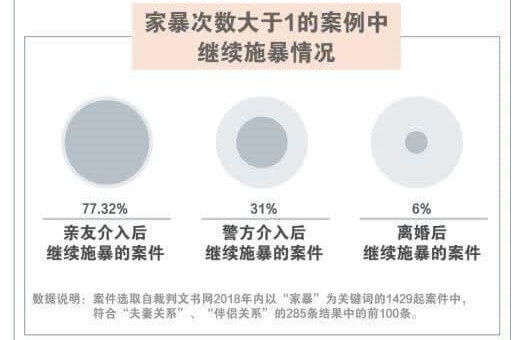
\includegraphics[height=.5\textheight]{../docs/img/3-9.jpg}
        \hfill
        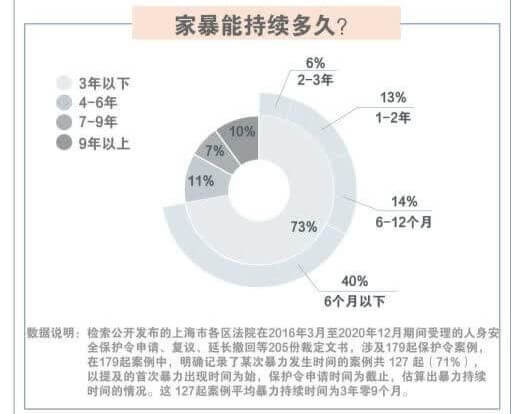
\includegraphics[height=.5\textheight]{../docs/img/3-10.jpg}
    \end{block}
\end{frame}

\begin{frame}{家庭暴力的受害者以女性为主}
    \begin{block}{}
        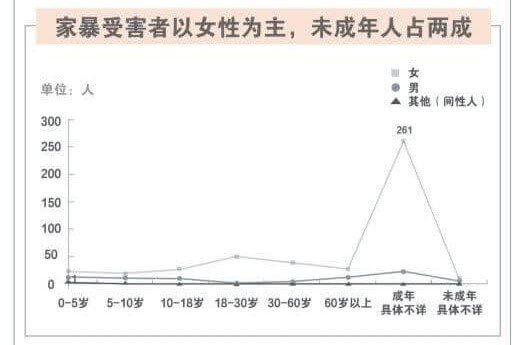
\includegraphics[height=.5\textheight]{../docs/img/3-11.jpg}
        \hfill
        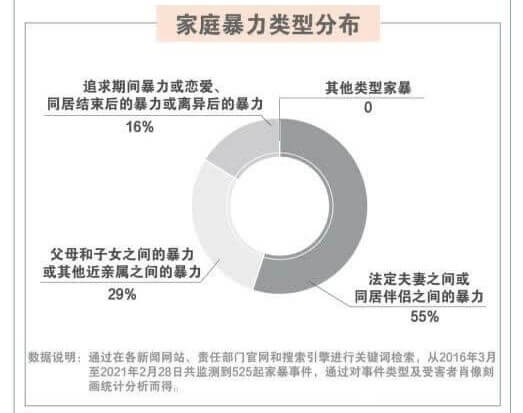
\includegraphics[height=.5\textheight]{../docs/img/3-12.jpg}
    \end{block}
\end{frame}

\begin{frame}{家庭暴力}
    \begin{block}{}
        当女性受到家暴时,女性或许会试图离婚,这里,虽然\textbf{离婚冷静期的存在仅仅是制约了协议离婚},可想要企图通过诉讼的方式,一次判决离婚成功仍然非常困难,因为\textbf{法院判定离婚的标准是“夫妻感情是否确已破裂”,这其中可能会伴随着各种导致判决失败的因素,像是证据不充分等等}。因此,在这样的社会背景下,一部分人会选择忍受不堪。但这也可能会带来一系列后果,甚至可能会引起社会恐慌。在这一方面,显然,以他人评价为导向的社会风气亟待改变,而相关的法律法规也需进一步完善。
    \end{block}
\end{frame}

\begin{frame}{家庭暴力}
    \begin{block}{}
        这里我们有一个例子,河南商丘一女子先后三次遭受丈夫的家庭暴力,第二次暴力直接导致了该女子用跳楼的方式逃生。前两次家暴,在婆婆和丈夫的软磨硬泡下,该女子都选择了原谅。而法院在第三次家暴发生近一年后,开庭审理离婚案件。可该女子却被告知因男方希望调解以及家暴事实不确定等原因,无法立刻判决。我们希望,法律应当更加健全,至少让受害者看到希望,而让家暴者也能得到相应的惩罚。
    \end{block}
    \begin{center}
        
\includegraphics[width=.9\textwidth]{../docs/img/3-7.jpg}
        
\includegraphics[width=.9\textwidth]{../docs/img/3-8.jpg}
    \end{center}
\end{frame}



\subsection{性安全方面}
\begin{frame}{性骚扰、性侵害}
    \begin{block}{}
        
\includegraphics[height=.55\textheight]{../docs/img/3-4.jpg}
        
\includegraphics[height=.55\textheight]{../docs/img/3-5.jpg}
        
\includegraphics[height=.55\textheight]{../docs/img/3-6.jpg}
    \end{block}
\end{frame}

\begin{frame}{性安全}
    \begin{block}{}
        我们知道,性骚扰、性侵害都是损害妇女 性权利的行为。类似的,我们发现当今社会,女性群体仍然没有足够高的保留性侵犯相关证据的意识。即使存在证据,相当一部分人也会羞于提起诉讼,其一部分原因是受到侵害伊始,自卑与自我厌恶便可能一直伴随于其身边,女性可能难以承受来自社会舆论的压力,又或是顾忌周围交际圈中的人情关系;另一部分原因则是由于我国民法法律体系在构建精神损害赔偿相关内容的缺失。可以看到,刑事诉讼法仍然规定被害人因犯罪行为遭受精神损失而提起附带民事诉讼的,法律规定人民法院不予受理。而民法典中侵害生命权、健康权和身体权的精神损害赔偿则尚未出台,仅仅是侵犯人身自由可以给予相关补偿。\textbf{这里,立法者倾向于认为侵害妇女性权利的法律保护 能包括民事法律保护是一个道德法律悖论与荒谬的问题,它有悖于现代道德观念,却也是一个法律悖论。}因此,不应当存在因性侵犯请求赔偿的相关法律依据。

        \textbf{因此,我国当前仍然需要在社会舆论环境构建和司法体系建设这两个方向上取得进步,从而提供给女性一个更加灵活且温和的空间以维护自身合法权利。}
    \end{block}
\end{frame}
